\documentclass[11pt, a4paper]{article}

\usepackage[T1]{fontenc}
\usepackage[utf8]{inputenc}

\usepackage{verbatim}
\usepackage{amsmath}
%\usepackage{biblatex} 
\usepackage{graphicx}   
\usepackage{float}
\usepackage{appendix}   
\usepackage{listings}   
\usepackage{xcolor}
\usepackage{siunitx}
\usepackage{pdfpages}
\usepackage{textcomp, gensymb}
\usepackage{multirow}

\sisetup{detect-all}

\usepackage[
backend=biber,
style=ieee,
sorting=ynt
]{biblatex}

\addbibresource{1.bib}

\title{Power Electronics - 12V Universal Supply \\ Design and Measurement Report}
\author{Jorge Pais \\ Ranlin Huang \\ Samriddha Ray }
\date{December 2023}

\begin{document}

\maketitle
\vfill \pagebreak
\tableofcontents
\vfill \pagebreak

\section{Introduction/Specification}

Our project proposed for the power electronics course unit was the universal 12V power supply. The original specifications were as follows:

\begin{itemize}
    \item Output voltage: 12V
    \item Input voltage : min. 5V; max. 18V
    \item Output Current: 1A 
\end{itemize}

Considering these, the team attempted to overdimension the circuit in order to output more current (2A) and accept a higher range of input voltages (min. 5V and max. 24V).

\section{Design}

\subsection{Circuit}

As the basis for the design, the LM5175 buck-boost converter controller by Texas Instruments \cite{lm7175data} was chosen. Since the design requires 2A of output current, a externally switched solution is a safer approach and as such the LM5175 presents a relatively modern design without many features such as $\text I^2\text C$ that would not be utilized. Also the four switch buck-boost converter approach as some advantages over traditional single or dual switch topologies, since at any given time two of the MOSFETs are in either on or off state while the other commutate. This has the benefit that no diodes are needed, and thus lower forward voltage drops are present in both modes of operation.

An example circuit schematic for the circuit can be seen in figure \ref{fig:exampleSchem}. The circuit developed is based around this initial design and uses follows the dimensioning procedure that is described in the IC's datasheet \cite{lm7175data}.

\begin{figure}[H]
    \centering
    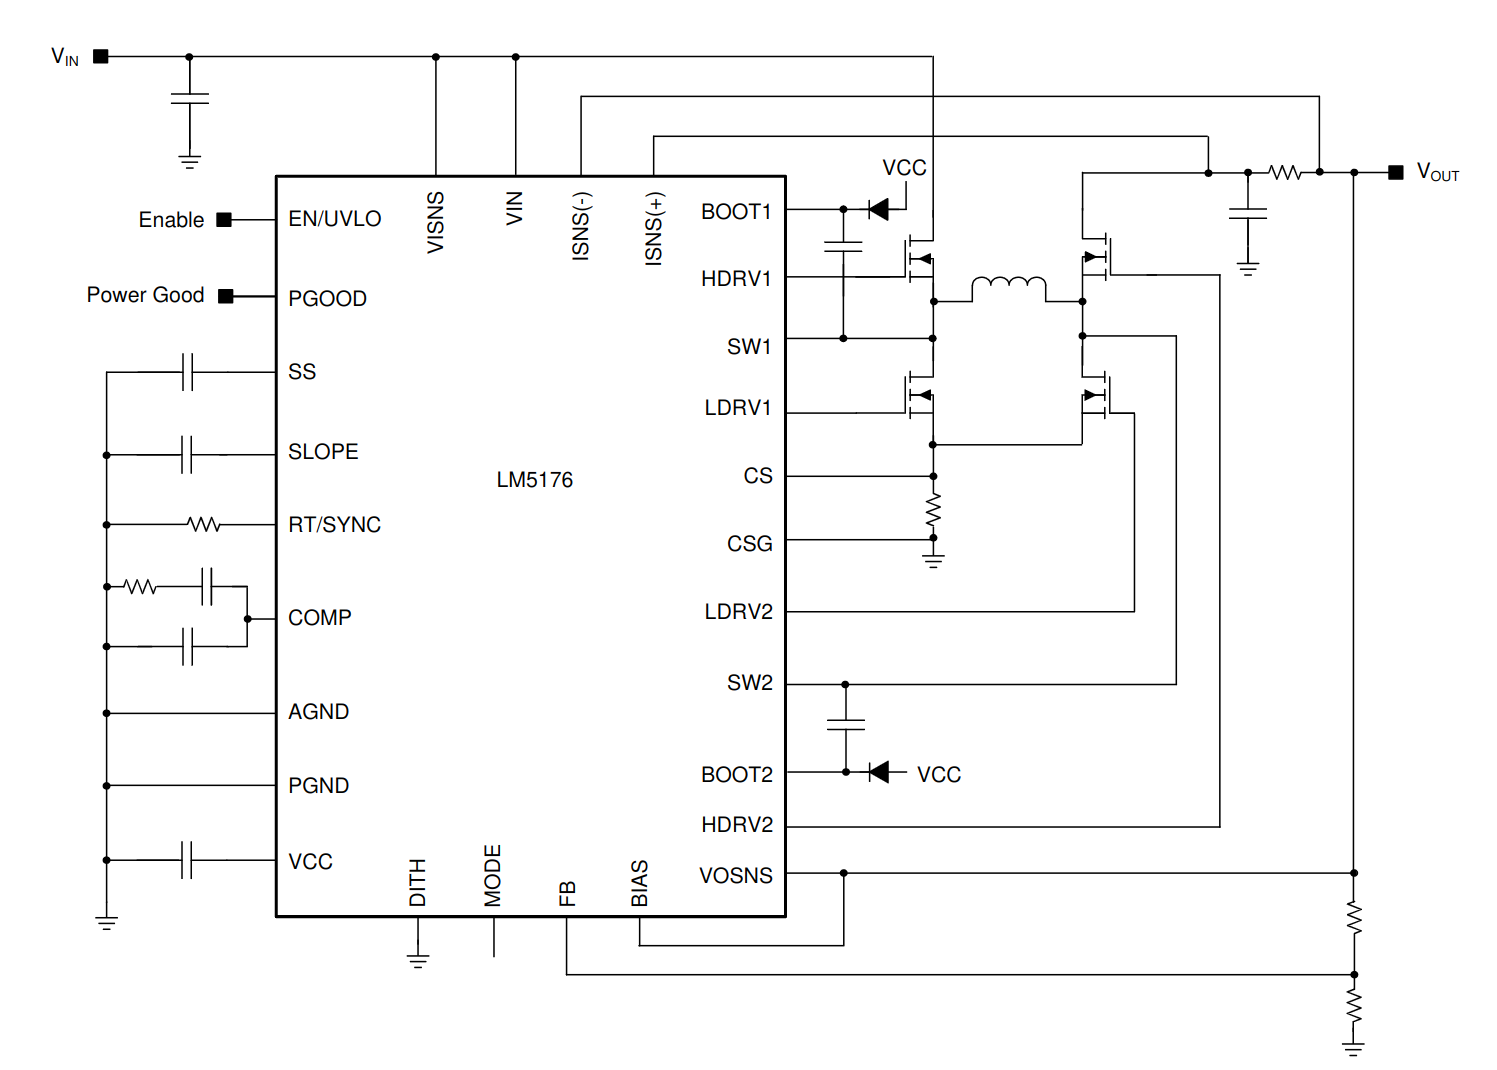
\includegraphics[width=0.8\textwidth]{figures/exampleSchematic.png}
    \caption{Simplified LM5175 Schematic}
    \label{fig:exampleSchem}
\end{figure}

As for the final schematic, a simplified version without connectors and testpoints can be found at the end of this document as an appendix.

\subsubsection{Switching Frequency}

The LM5175's switching frequency can be programmed between 100 and 600 kHz using a resistor from the RT/SYNC pin to ground. Higher values lead to higher overall efficiency but with added EMI and noise. The switching frequency was chosen to be 300kHz, as most examples featured in the datasheet used this value.

\begin{equation}
    R_T = \frac{1/F_{SW}-190\text{ns}}{116\text{pF}} = 27.4 \text k \Omega
\end{equation}

\subsubsection{Feedback Network}

The output voltage of the circuit is set using a the feedback network between the output and the IC's FB pin. 

\begin{equation}
    \frac{R_{FB2}}{R_{FB1}} = \frac{V_{out}-0.8}{0.8} = 14
\end{equation}

Choosing E48 series resistor values, a perfect ratio can be obtained:

$$R_{FB1} = 7.5 \text k \Omega; R_{FB2} = 105 \text k \Omega$$

\subsubsection{Inductor Selection}

The target inductance for Buck mode is given by the following formula:

\begin{equation}
    L_{buck} = \frac{(V_{inMAX}-V_{out})V_{out}}{0.4I_{outMAX}F_{SW}V_{inMAX}} = 25 \mu \text H
\end{equation}

And the target for boost mode is the following:

\begin{equation}
    L_{boost} = \frac{V_{inMIN}^2 (V_{out}-V_{inMIN})}{0.3I_{outMAX}F_{SW}V_{out}^2}= 4.93 \mu \text H
\end{equation}

The maximum average inductor current is the following if we assume 90\% efficiency:

\begin{equation}
    I_{Lmax} = \frac{V_{out}I_{outMAX}}{0.9V_{inMIN}}= 6.66\text A
\end{equation}

Given this, the datasheet actually under specifies this component. A $4.7\mu \text H$ inductor can be utilized and as such, the XAL1010-472MED from Coilcraft \cite{XAL1010data} was chosen.

As for the peak inductor following through the inductor it is:

\begin{equation}
    I_{Lpeak} = I_{Lmax} + \frac{V_{inMIN}(V_{out}-V_{inMIN})}{2L_1F_{sw}V_{out}} \approx 6.66 \text A  
\end{equation}

\subsubsection{Output Capacitors}

The value for the main output capacitor can be determined by the capacitive ripple voltage:

\begin{equation}
    \Delta V_{ripple} = \frac{I_{out}(1-\frac{V_{inMIN}}{V_{out}})}{C_{out}F_{SW}}
\end{equation}

And so, for a 10mV ripple from the capacitor, a value of $444.44\mu \text F$ is required. As such $C_{out} = 470\mu \text F$, which can be achieved with a small electrolytic capacitor. For this purpose Panasonic's 25SPVK470M Polymer Aluminum capacitor was chosen, which has a maximum voltage rating of 25V and a ESR of 14m$\Omega$.

Along side this, three smaller $15\mu \text F$ tantalum capacitors are placed in parallel, such as to minimize output ESR. So, the TPSA156K006R0700 from Kyocera Avx was chosen, each featuring an ESR of 7m$\Omega$. 

For the boost mode of operation the RMS current through the capacitor is given by:

\begin{equation}
    I_{Cout_{RMS}} = I_{out} \sqrt{\frac{V_{out}}{V_{in}}-1}
    \label{eq:coutIrms}
\end{equation}

\subsubsection{Input Capacitors}

As for the input capacitors, in the buck operating region, they need to be able to supply high ripple current. It's RMS current is given by the following equation, where the worst case scenario of D = 0.5 should be considered:

\begin{equation}
    I_{C_{in}rms} = I_{out} \sqrt{D(1-D)} = 1 A
    \label{eq:cinIrms}
\end{equation}

So in a similar fashion as for the output, a bulk electrolytic capacitor of $68\mu \text F$ was placed in parallel with several $15\mu \text F$ tantalum capacitors. The bulk capacitor chosen was the Panasonic EEHZT1J680P featuring a maximum voltage rating of 63V and a ESR of 25m$\Omega$.

\subsubsection{Current Limit}

The circuit's current limit is set by the $R_{sense}$ resistor at the tail of the 4 mosfet switch bridge.

\begin{equation}
    R_{senseBUCK} = \frac{80\text{mV}}{I_{outMAX}} = 40\text m\Omega
\end{equation}

\begin{equation}
    R_{senseBOOST} = \frac{120\text{mV}}{I_{Lpeak}} = 18\text m\Omega
\end{equation}

This value is then set to $R_{sense} = 18\text m\Omega$ based on the boost mode operation. The power loss experienced by the $R_{sense}$ is the following:

\begin{equation}
    P_{senseMAX} = \left (\frac{120mV}{R_{sense}}\right )^2R_{sense}\left (1-\frac{V_{inMIN}}{V_{out}}\right ) = 0.53 \text W
    \label{eq:rsensePower}
\end{equation}

Hence a 1W sense resistor is sufficient. As for the sense lines $R_{CS}$ and $R_{CSG}$ the values were chosen according to the example schematic provided on the datasheet: $R_{CS} = R_{CSG} = 100\Omega$. A filter capacitor is also needed to attenuate the noise that can occur in these lines due to the large amounts of current passing through $R_{sense}$, as such a 47pF capacitor is utilized as a part of a differential mode filter in the CS and CSG pins to the LM5175.

\subsubsection{MOSFETs}

The LM5175 features four built-in N-channel MOSFET gate drivers. In buck operation, QL1 and QH1 are switched by the IC's PWM controller while QH2 is continuously on and QL2 off. As for boost operation, QL2 and QH2 are switching while QH1 remains continuously on and QL2 is off.

For the QH1 and QL2 MOSFETs on the input side, these need to withstand the maximum input voltage of the circuit, plus the possible voltage transient spikes. Considering the extended specifications, this value comes to $V_{DS_{max}} \ge 24 + 20V$. As for the output, transistors QH2 and QL2 should be rated for 12V plus the transient spikes.

When choosing a MOSFET for this circuit, it is also important to consider the rise/fall time and gate charges of the transistor, in order to minimize switching time and thus minimize switching loss. Also, the drain-to-source on-resistance should be minimal in order to lower the conduction losses.

Considering these requirements, the MOSFET chosen for the 4 switches was the Texas Instruments' CSD18532Q5B n-channel MOSFET \cite{CSD18532data}, claiming to feature maximum $V_{gs}$ of 60V and ultra-low gate charges.

\subsubsection{Frequency Compensation}

At the maximum load of 2A, output resistance is $R_{out} = V_{out}/I_{outMAX} 6\Omega$

\begin{equation}
    f_{p1(boost)} = \frac{2}{2\pi R_{out}C_{out}} = 112 \text{Hz}    
\end{equation}

\begin{equation}
    f_{z1} = \frac{1}{2\pi R_{esr}C_{out}} = 226 \text{Hz}    
\end{equation}

The boost power stage RHP zero location is given by: 

\begin{equation}
    f_{RHP} = \frac{R_{out}(1-D_{max})^2}{2\pi L_1} = 22.57\text{kHz}
\end{equation}

Where $D_{max}$ is the maximum duty cycle at the minimum $V_{in}$: $D = 1-\frac{V_i}{V_o} = 0.667$ 

\begin{equation}
    f_{p1(buck)} = \frac{1}{2\pi R_{out}C_{out}} = 56.4379  
\end{equation}

From these, it is clear that the RHP zero is the main factor limiting the achievable bandwidth.

\begin{equation}
    f_{bw} = \frac{f_{RHP}}{3} = 7.52\text{kHz}    
\end{equation}

The compensation zero can be placed at 1.5 times the boost frequency pole.

\begin{equation}
    f_{zc} = 1.5f_{p1(boost)} = 168\text{Hz}  
\end{equation}

Then the values for $R_{c1}, C_{c1}$ and $C_{c2}$ can be figured out through the following expressions:

\begin{equation}
    R_{c1} = \frac{2\pi f_{bw}}{gm_{EA}}\frac{R_{FB1}+R_{FB2}}{R_{FB1}}\frac{A_{cs}R_{sense}C_{out}}{1-D_{max}} = 68656\Omega \approx 68\text k \Omega  
\end{equation}

\begin{equation}
    C_{c1} = \frac{1}{2\pi f_{zc} R_{c1}} = 13.79 \text{nF} \approx 13 \text{nF}    
\end{equation}

\begin{equation}
    C_{c2} = \frac{1}{2\pi 5 f_{bw} R_{c1}} = 61.65 \text{pF} \approx 62 \text{pF}    
\end{equation}

\subsubsection{Boilerplate Circuitry}

In order to turn-on the IC, an appropriate voltage divider has to be built around the Enable/UVLO pin of the LM5175, which also functions as an undervoltage lockout, providing hysteresis between the turn-on and turn-off voltages. Using the following equation, the E96 values for the resistors can be calculated:

\begin{eqnarray}
    \begin{cases}
        V_{UV} = V_{en} \left (1 + \frac{R_{UV1}}{R_{UV2}}\right ) - R_{UV2}I_{en} \\
        R_{UV1} = 59\text k\Omega; R_{UV1} = 249\text k\Omega 
    \end{cases}
\end{eqnarray}

The LM5175 also features what is called soft start, which charges an external capacitor whenever the converter is powered up, replacing the internal reference voltage for the feedback in the error amplifier. Once fully charged, the internal error amplifier is then referenced to $V_{ref}$ again.

A 20ms soft-start should be plenty for this circuit:

\begin{equation}
    \begin{cases}
        I_{ss} = 5\mu \text A \\        
        C_{ss} = \frac{t_{ss}I_{ss}}{V_{ref}} = 125 \text{nF} \approx 120 \text{nF} \\
    \end{cases}
\end{equation}

Apart from the frequency compensation dimensioned previously, slope compensation is also an important step in the design of any current-mode controlled converters in order to avoid oscillations. For the case of the LM5175 it should be dimensioned as such:

\begin{equation}
    C_{slope} = g_{m_{slope}}\frac{L1}{R_{sense}A_{cs}} = 100\text{pF}    
\end{equation}

Finally, the bootstrap capacitors and diodes also have to be chosen in order for the integrated MOSFET drivers to function as intended. For this purpose, 100nF ceramic caps were chosen. Also the SS24 Schottky Barrier Rectifier by Multicomp Pro was decided upon for the diodes due to it's 2A forward current and 40V peak reverse voltage \cite{SS24data}. It doesn't matter all that much as long as it's a schottky, but this diode was chosen also because it could withstand the possible peak voltages from the MOSFET bridge, and reusing it throughout the circuit reduces the final BOM. 

\subsection{Power Losses \& Efficiency}

\subsubsection{MOSFETs}

In the buck mode of operation, the conduction and switching losses are given by the following formulas \cite{lm7175data}:

\begin{equation}
    \begin{cases}
        P_{cond(QH1)} = \frac{V_{out}}{V_{in}}I_{out}^2 R_{DSon} \\
        P_{SW(QH1)} = \frac{1}{2}V_{in}I_{out}(t_r + t_f)F_{SW} \\
        P_{cond(QL1)} = \left (1-\frac{V_{out}}{V_{in}} \right ) I_{out}^2 R_{DSon} \\
        P_{cond(QH2)} = I_{out}^2R_{DSon}
    \end{cases}
\end{equation}

As for when the converter is operating in boost mode:

\begin{equation}
    \begin{cases}
        P_{cond(QH1)} = \left (\frac{V_{out}}{V_{in}}I_{out} \right )^2 R_{DSon} \\
        P_{cond(QL2)} = \left (1 - \frac{V_{out}}{V_{in}}\right ) \left (\frac{V_{out}}{V_{in}}I_{out} \right )^2 R_{DSon} \\
        P_{SW(QL2)} = \frac{1}{2}V_{out}\left (\frac{V_{out}}{V_{in}}I_{out} \right )(t_r + t_f)F_{SW} \\
        P_{cond(QH2)} = \frac{V_{in}}{V_{out}}\left (I_{out}\frac{V_{out}}{V_{in}} \right )^2 R_{DSon}
    \end{cases}
\end{equation}

If we plug some of the datasheet specifications into the power loss equations, along with the worst case values for $V_{in}$ and $I_{out}$ then the results on table \ref{tab:mosfetLosses} are obtained. It should be taken into account that the actual rise/fall switching times have to be determined empirically in the lab, so the values used consider a much higher current than what our circuit consumes.

\begin{table}[H]
    \centering
    \begin{tabular}{|c|c|c|c|}
        \hline
        \multicolumn{2}{|c|}{Buck} & \multicolumn{2}{|c|}{Boost} \\
        \hline \hline
        $P_{cond(QH1)}$ & $8.6$mW  & $P_{cond(QH1)}$ & $99.1$mW \\
        $P_{SW(QH1)}$   & $74.2$mW & $P_{cond(QL2)}$ & $57.8$mW \\
        $P_{cond(QL1)}$ & $8.6$mW  & $P_{SW(QL2)}$   & $59.4$mW \\
        $P_{cond(QH2)}$ & $17.2$mW & $P_{cond(QH2)}$ & $41.3$mW \\
        \hline
    \end{tabular}
    \caption{Maximum MOSFET Power Losses}
    \label{tab:mosfetLosses}
\end{table}

From these it is also to obtain an idea of the thermal performance of these MOSFETs (table \ref{tab:mosfetTemp}), which even at 2A barely heat up indicating very strong efficiency. This is mostly due to the transistors chosen having both very low gate charges and low $R_{DSon}$.

\begin{table}[H]
    \centering
    \begin{tabular}{|c|c|}
        \hline
        \multirow{2}*{Transistor} & Temperature \\
         & Rise $\Delta T (\degree C)$ \\
        \hline \hline
        $QH1_{Buck}$  & $4.14$ \\
        $QL1_{Buck}$  & $0.43$ \\
        $QH2_{Buck}$  & $0.86$ \\
        $QH1_{Boost}$ & $4.96$ \\
        $QL2_{Boost}$ & $5.86$ \\
        $QH2_{Boost}$ & $2.07$ \\
        \hline
    \end{tabular}
    \caption{Junction-ambient temperature rise}
    \label{tab:mosfetTemp}
\end{table}

Figures \ref{fig:mosfetBuckLosses} and \ref{fig:mosfetBoostLosses} show how these losses are related to both the output current and varying input voltage.

\begin{figure}[H]
    \centering
    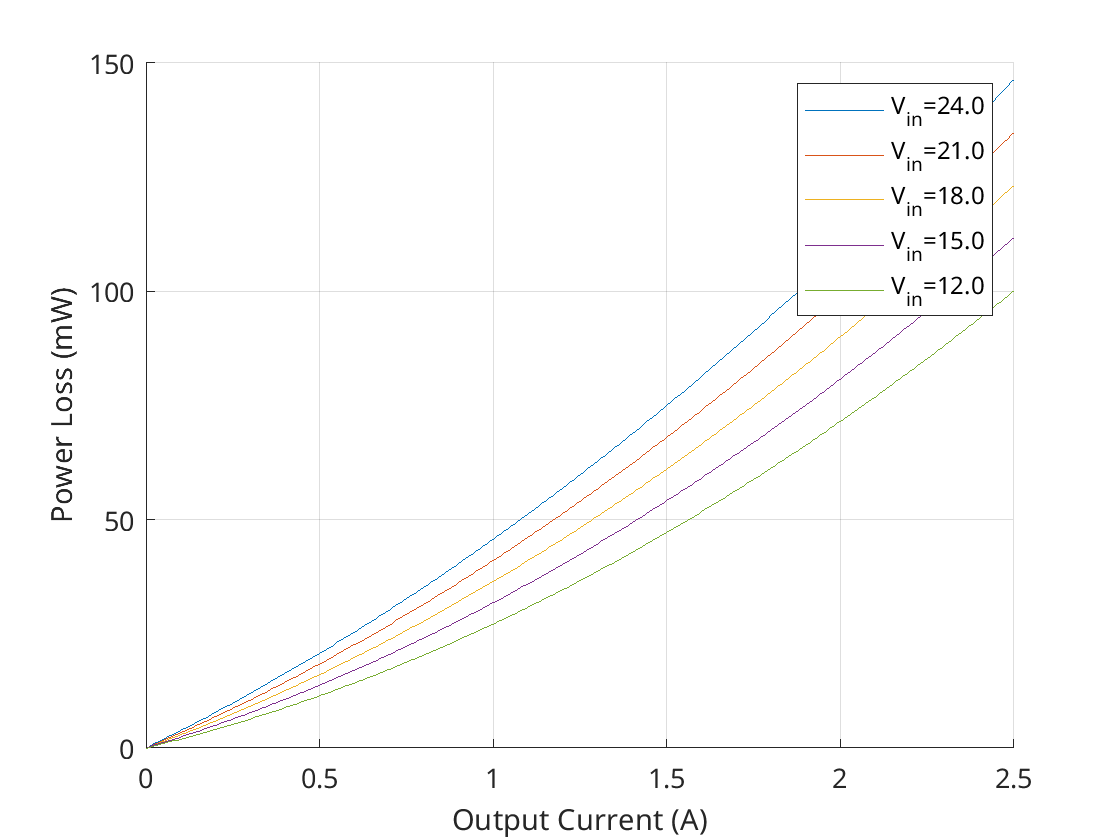
\includegraphics[width=0.6\textwidth]{./figures/mosfetBuckLosses.png}
    \caption{Buck mode MOSFET losses}
    \label{fig:mosfetBuckLosses}
\end{figure}

\begin{figure}[H]
    \centering
    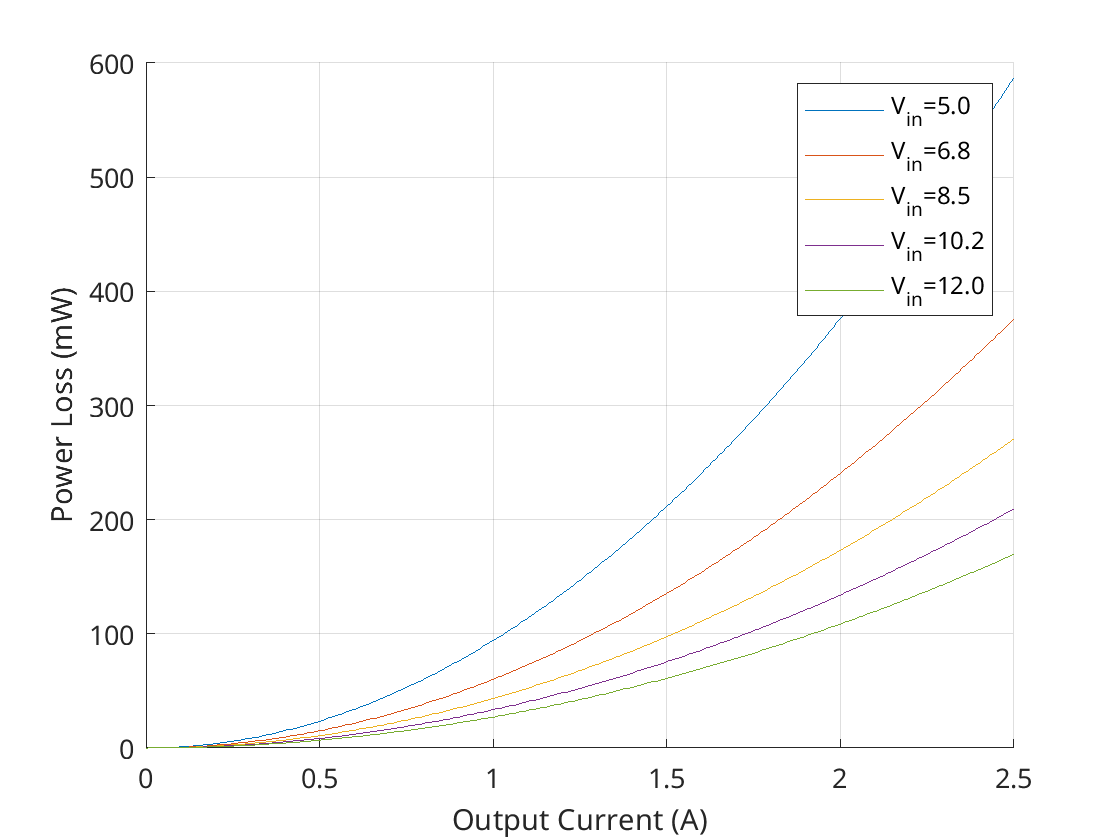
\includegraphics[width=0.6\textwidth]{./figures/mosfetBoostLosses.png}
    \caption{Boost mode MOSFET losses}
    \label{fig:mosfetBoostLosses}
\end{figure}

\subsubsection{Inductor}

Taking the formula for the RMS current through the inductor (with the previous assumption of 90\% efficiency, which certainly is a gross approximation especially when considering lower output currents), an estimate for dissipated power can be obtained if we consider the inductor's wire resistance $R_w = 5.70\text m\Omega$ \cite{XAL1010data}:

\begin{equation}
    P_{inductor} = I_{L_{RMS}}^2 R_w = \left (\frac{V_{out}I_{out}}{0.9V_{in}} \right )^2 R_w
\end{equation}

This gives a maximum power loss when the current is maximum and the input voltage is minimum, with a value of $P_{Lmax} = 162\text{mW}$. In figure \ref{fig:inductorLosses} we can observe the power loss in relation to the output current that is drawn from the converter, for varying input voltages.

\begin{figure}[H]
    \centering
    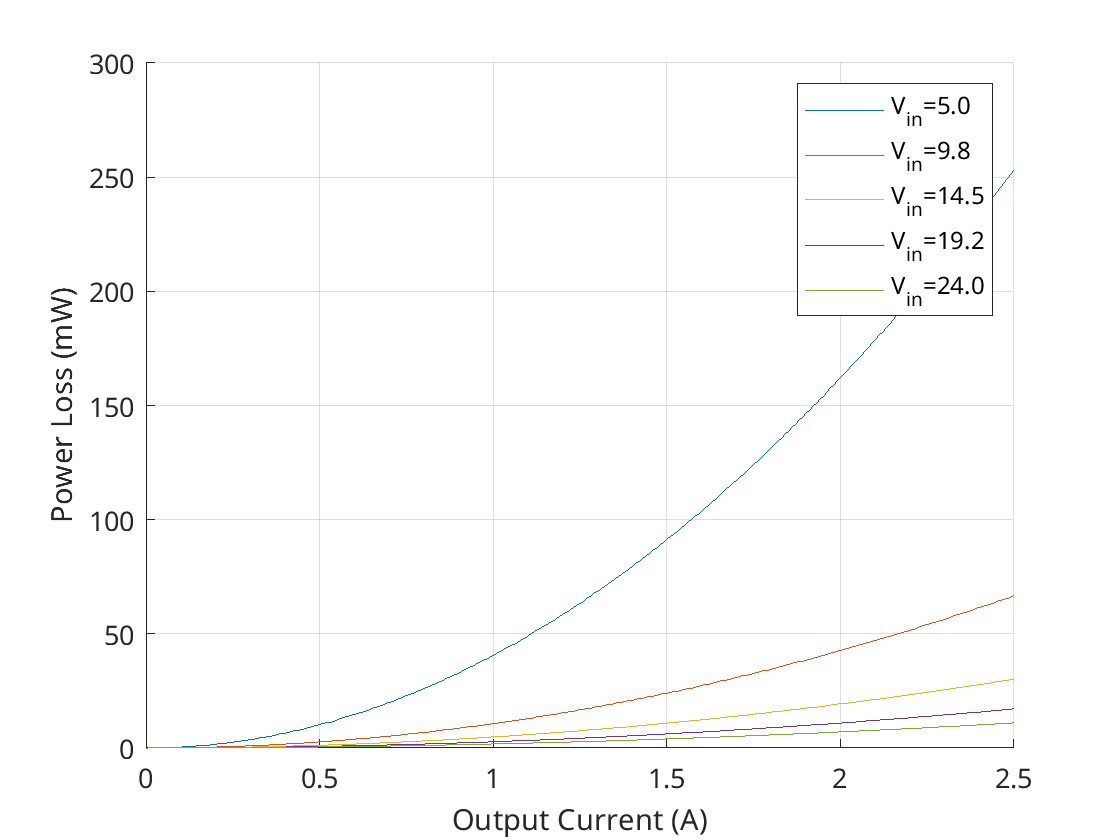
\includegraphics[width=0.6\textwidth]{./figures/inductorLosses.png}
    \caption{Inductor power losses}
    \label{fig:inductorLosses}
\end{figure}

\subsubsection{Capacitor Losses}

During the boost mode of operation the output capacitors are responsible for conducting high ripple current. Using formula \ref{eq:coutIrms} for the output current, capacitor buck-mode power losses can be estimated. The total ESR for the output capacitances is $ESR = 2.0\text m \Omega$.

\begin{equation}
    P_{C_{out}} = I_{C_{rms}}^2 ESR = I_{out}^2 \left (\frac{V_{out}}{V_{in}} - 1 \right ) ESR
\end{equation}

Figure \ref{fig:coutLosses} shows these losses as a function of the output current and the input voltage. It is possible to see that the biggest losses are when the input voltage is minimum where $P_{C_{out}} = 11\text{mW}$.

\begin{figure}[H]
    \centering
    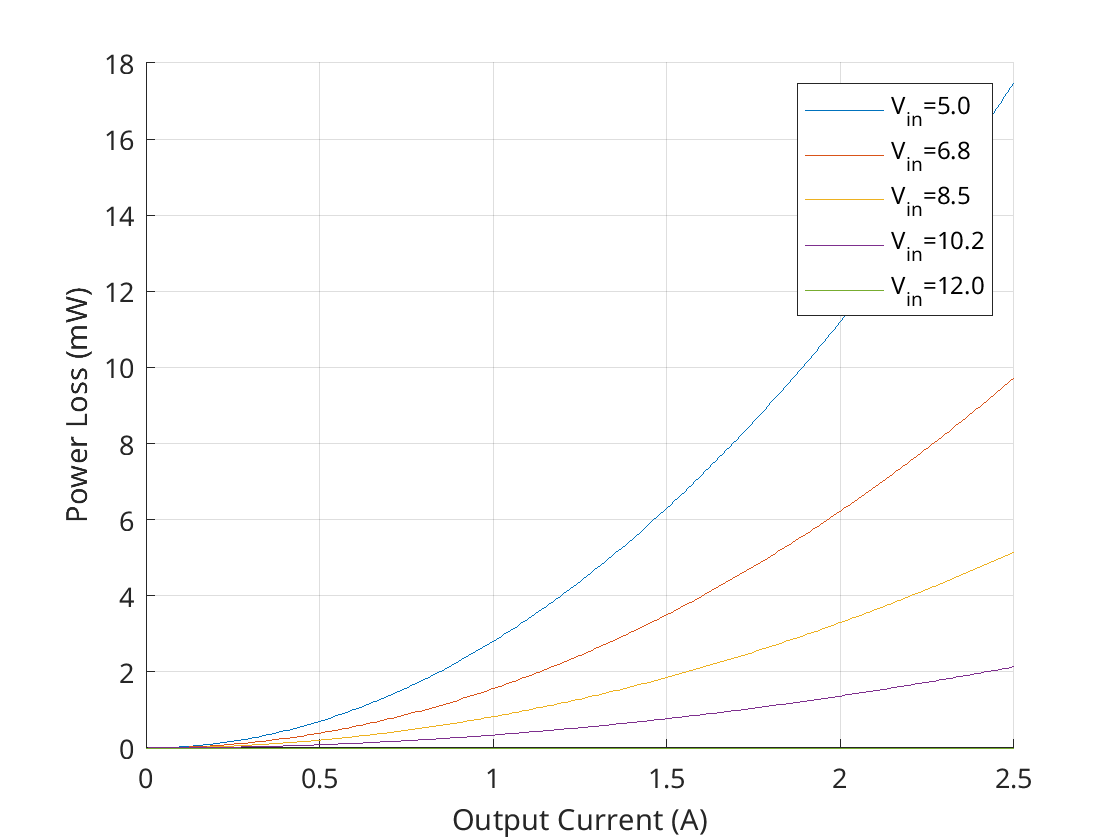
\includegraphics[width=0.6\textwidth]{./figures/outputCapLosses.png}
    \caption{Output capacitor power losses}
    \label{fig:coutLosses}
\end{figure}

As for the input capacitances, the formula for the RMS current in equation \ref{eq:cinIrms} can be utilized to figure out the power losses. The total ESR for the input capacitors is $2.13 \text m \Omega$.

\begin{equation}
    P_{C_{in}} = I_{C_{rms}}^2 ESR = I_{out}^2D(1-D)ESR
\end{equation}

Using this, figure \ref{fig:cinLosses} displays a plot of the power losses in respect to the output current. The maximum power loss is then obtained when the duty cycle is $D=0.5$, where $P_{C_{in}}=2.1\text{mW}$

\begin{figure}[H]
    \centering
    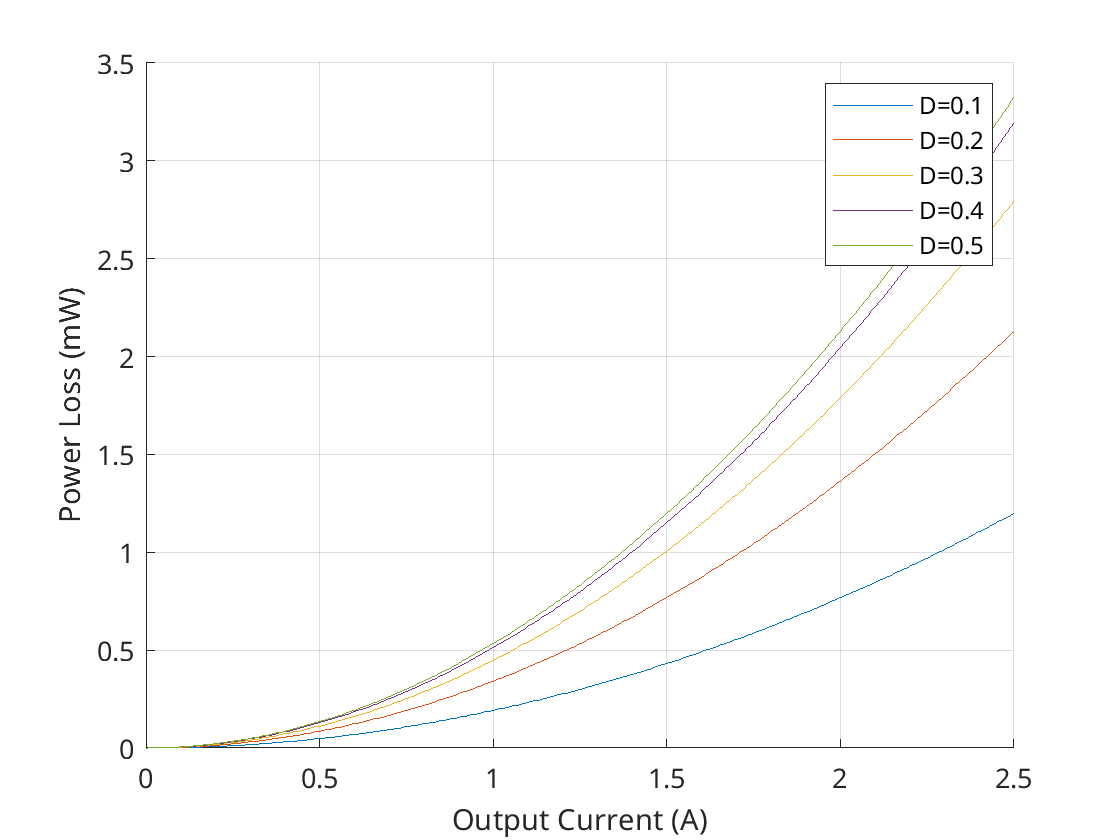
\includegraphics[width=0.6\textwidth]{./figures/inputCapLosses.png}
    \caption{Input capacitor power losses}
    \label{fig:cinLosses}
\end{figure}

\subsubsection{Sense resistor}

A formula for determining the power loss in $R_{sense}$ was already shown in equation \ref{eq:rsensePower}, but only for the boost mode. In this case the power loss was the following, in the worst case scenario:

$$P_{sense_{Boost}} = 530\text{mW}$$

For the buck mode, the formula is pretty much the same, only that the duty cycle is different and now we use the buck current limit threshold $V_{CS(BUCK)} = 80\text{mV}$ for the calculation.

\begin{equation}
    P_{sense_{Buck}} = \left (\frac{80mV}{R_{sense}}\right )^2R_{sense}\left (\frac{V_{out}}{V_{inMAX}}\right ) = 178 \text{mW}
\end{equation}

\subsubsection{Total Losses}

From the previous analysis, the total losses for each mode of operation can be calculated. Firstly the buck mode losses can be seen in figure \ref{fig:totalBuckLosses} which consider the worst case of $V_{in} = 24\text V$. 

\begin{figure}[H]
    \centering
    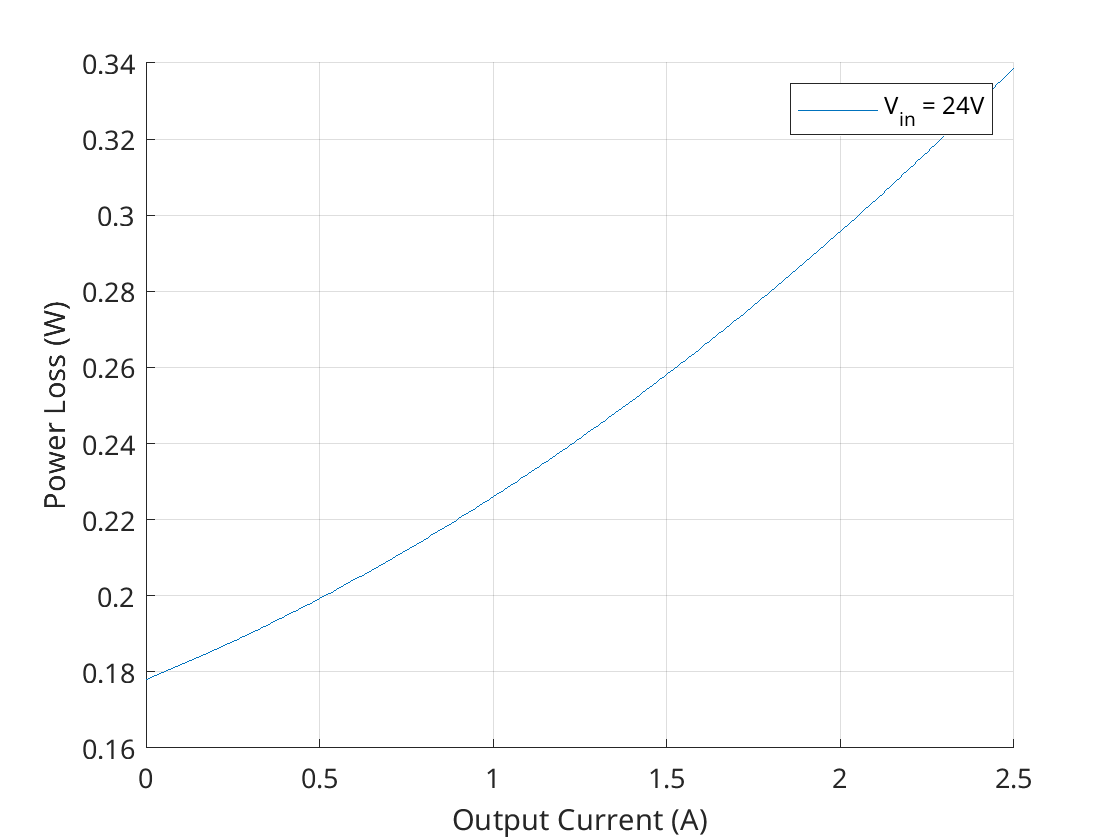
\includegraphics[width=0.6\textwidth]{./figures/totalBuckLosses.png}
    \caption{Total buck mode losses}
    \label{fig:totalBuckLosses}
\end{figure}

Figure \ref{fig:totalBoostLosses} shows the same, but for the boost mode of operation, in the worst case when the input voltage is 5V.

\begin{figure}[H]
    \centering
    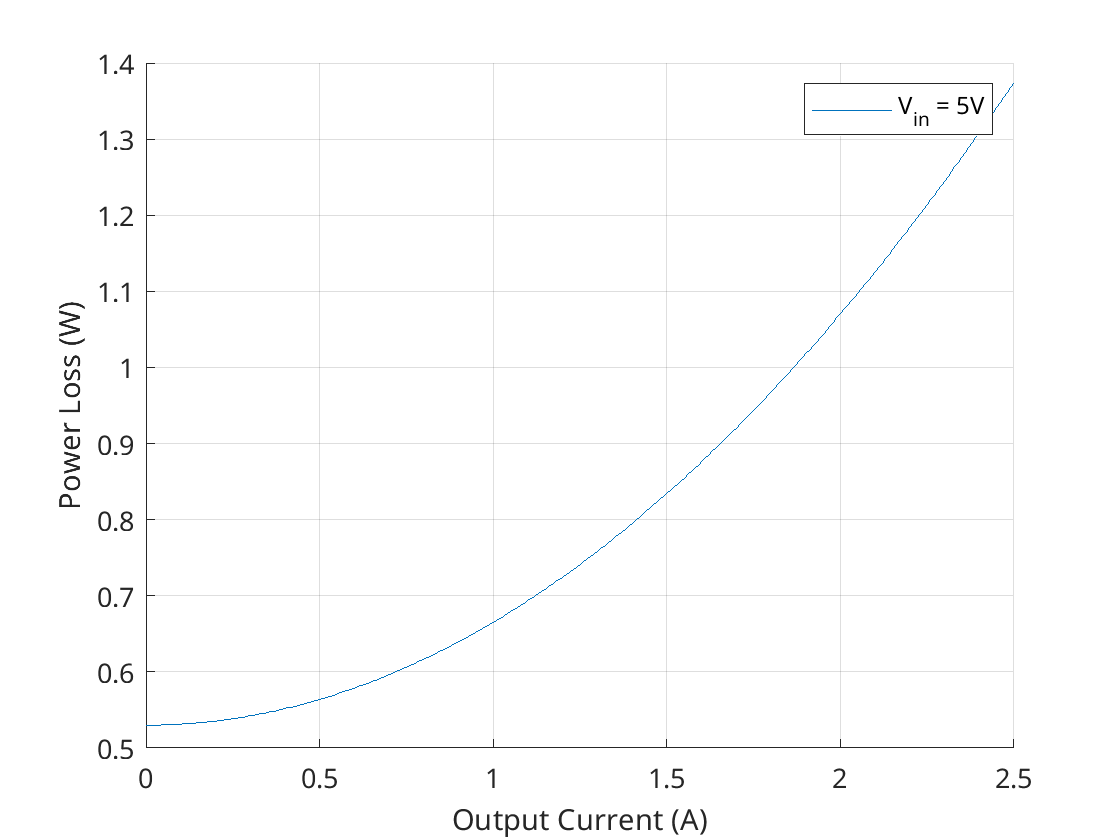
\includegraphics[width=0.6\textwidth]{./figures/totalBoostLosses.png}
    \caption{Total boost mode losses}
    \label{fig:totalBoostLosses}
\end{figure}

\subsubsection{Efficiency}

From the total losses, it is then possible to see what the theoretical efficiency of the converter is. Figure \ref{fig:efficiency} shows the worst case scenario efficiency for both the Boost and Buck modes ($V_{in} = 5\text V$ and $V_{in} = 24\text V$ respectively), as a function of output current.

\begin{figure}[H]
    \centering
    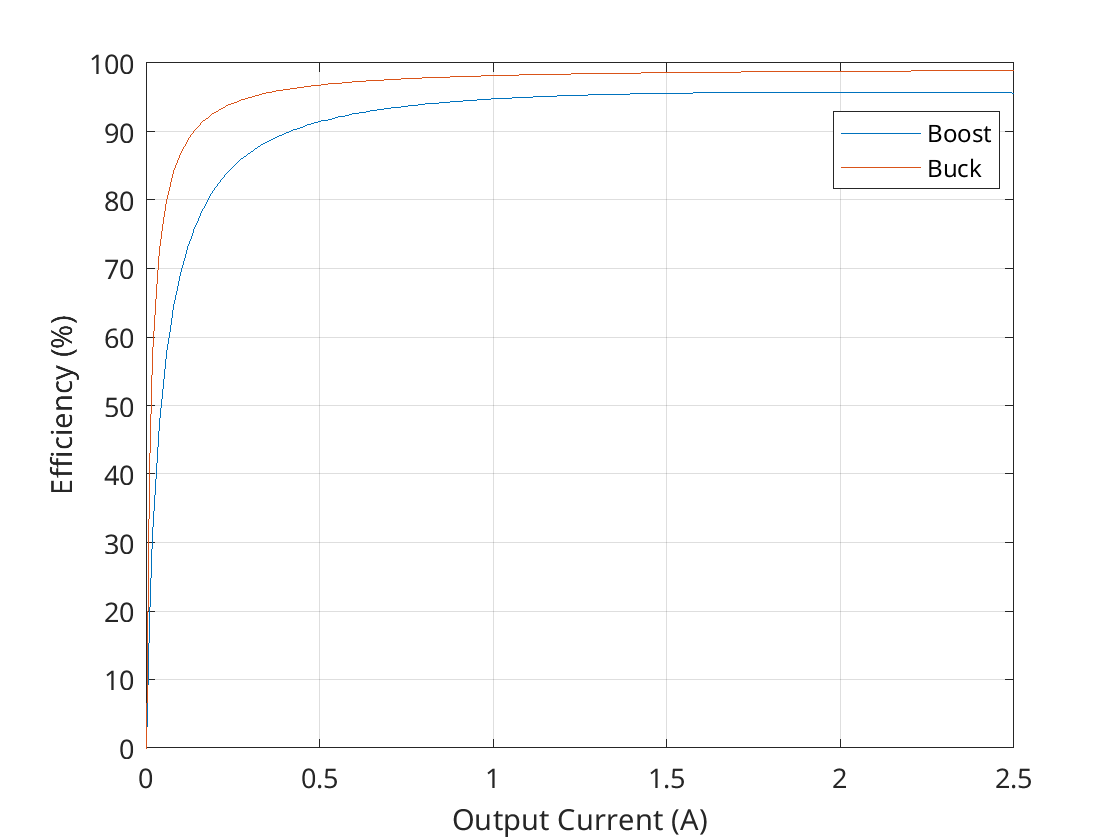
\includegraphics[width=0.6\textwidth]{./figures/efficiency.png}
    \caption{Buck and Boost efficiency}
    \label{fig:efficiency}
\end{figure}

\subsection{Board}

The board was designed utilizing KiCad 7 for both the schematic capture and PCB layout. Some of the specifications for the board were based on the project limitations and the constraints posed by JLCPCB manufacturing. These were was follows:

\begin{itemize}
    \item 2 layers, bottom GND plane
    \item SMD only, except for connectors/testpoints
    \item Min. copper clearence: 0.2mm
    \item Min. track width: 0.2mm
    \item Min. annular width: 0.13mm
    \item Min. via diameter: 0.7mm
    \item Min. copper to hole clearence: 0.25mm
    \item Min. through-hole diameter: 0.3mm
    \item Min. hole-to-hole clearence: 0.254mm
\end{itemize}

Considering these, a relatively simple and compact layout was achieved, whose routing can be seen in figure \ref{fig:pcbrouting}, without any of the filled zones to better visualize the trace routing. For this, the recommended layout for the LM5175 \cite{lm7175data} was used as a base, while following the remaining guidelines imposed by the manufacturer.

\begin{figure}[H]
    \centering
    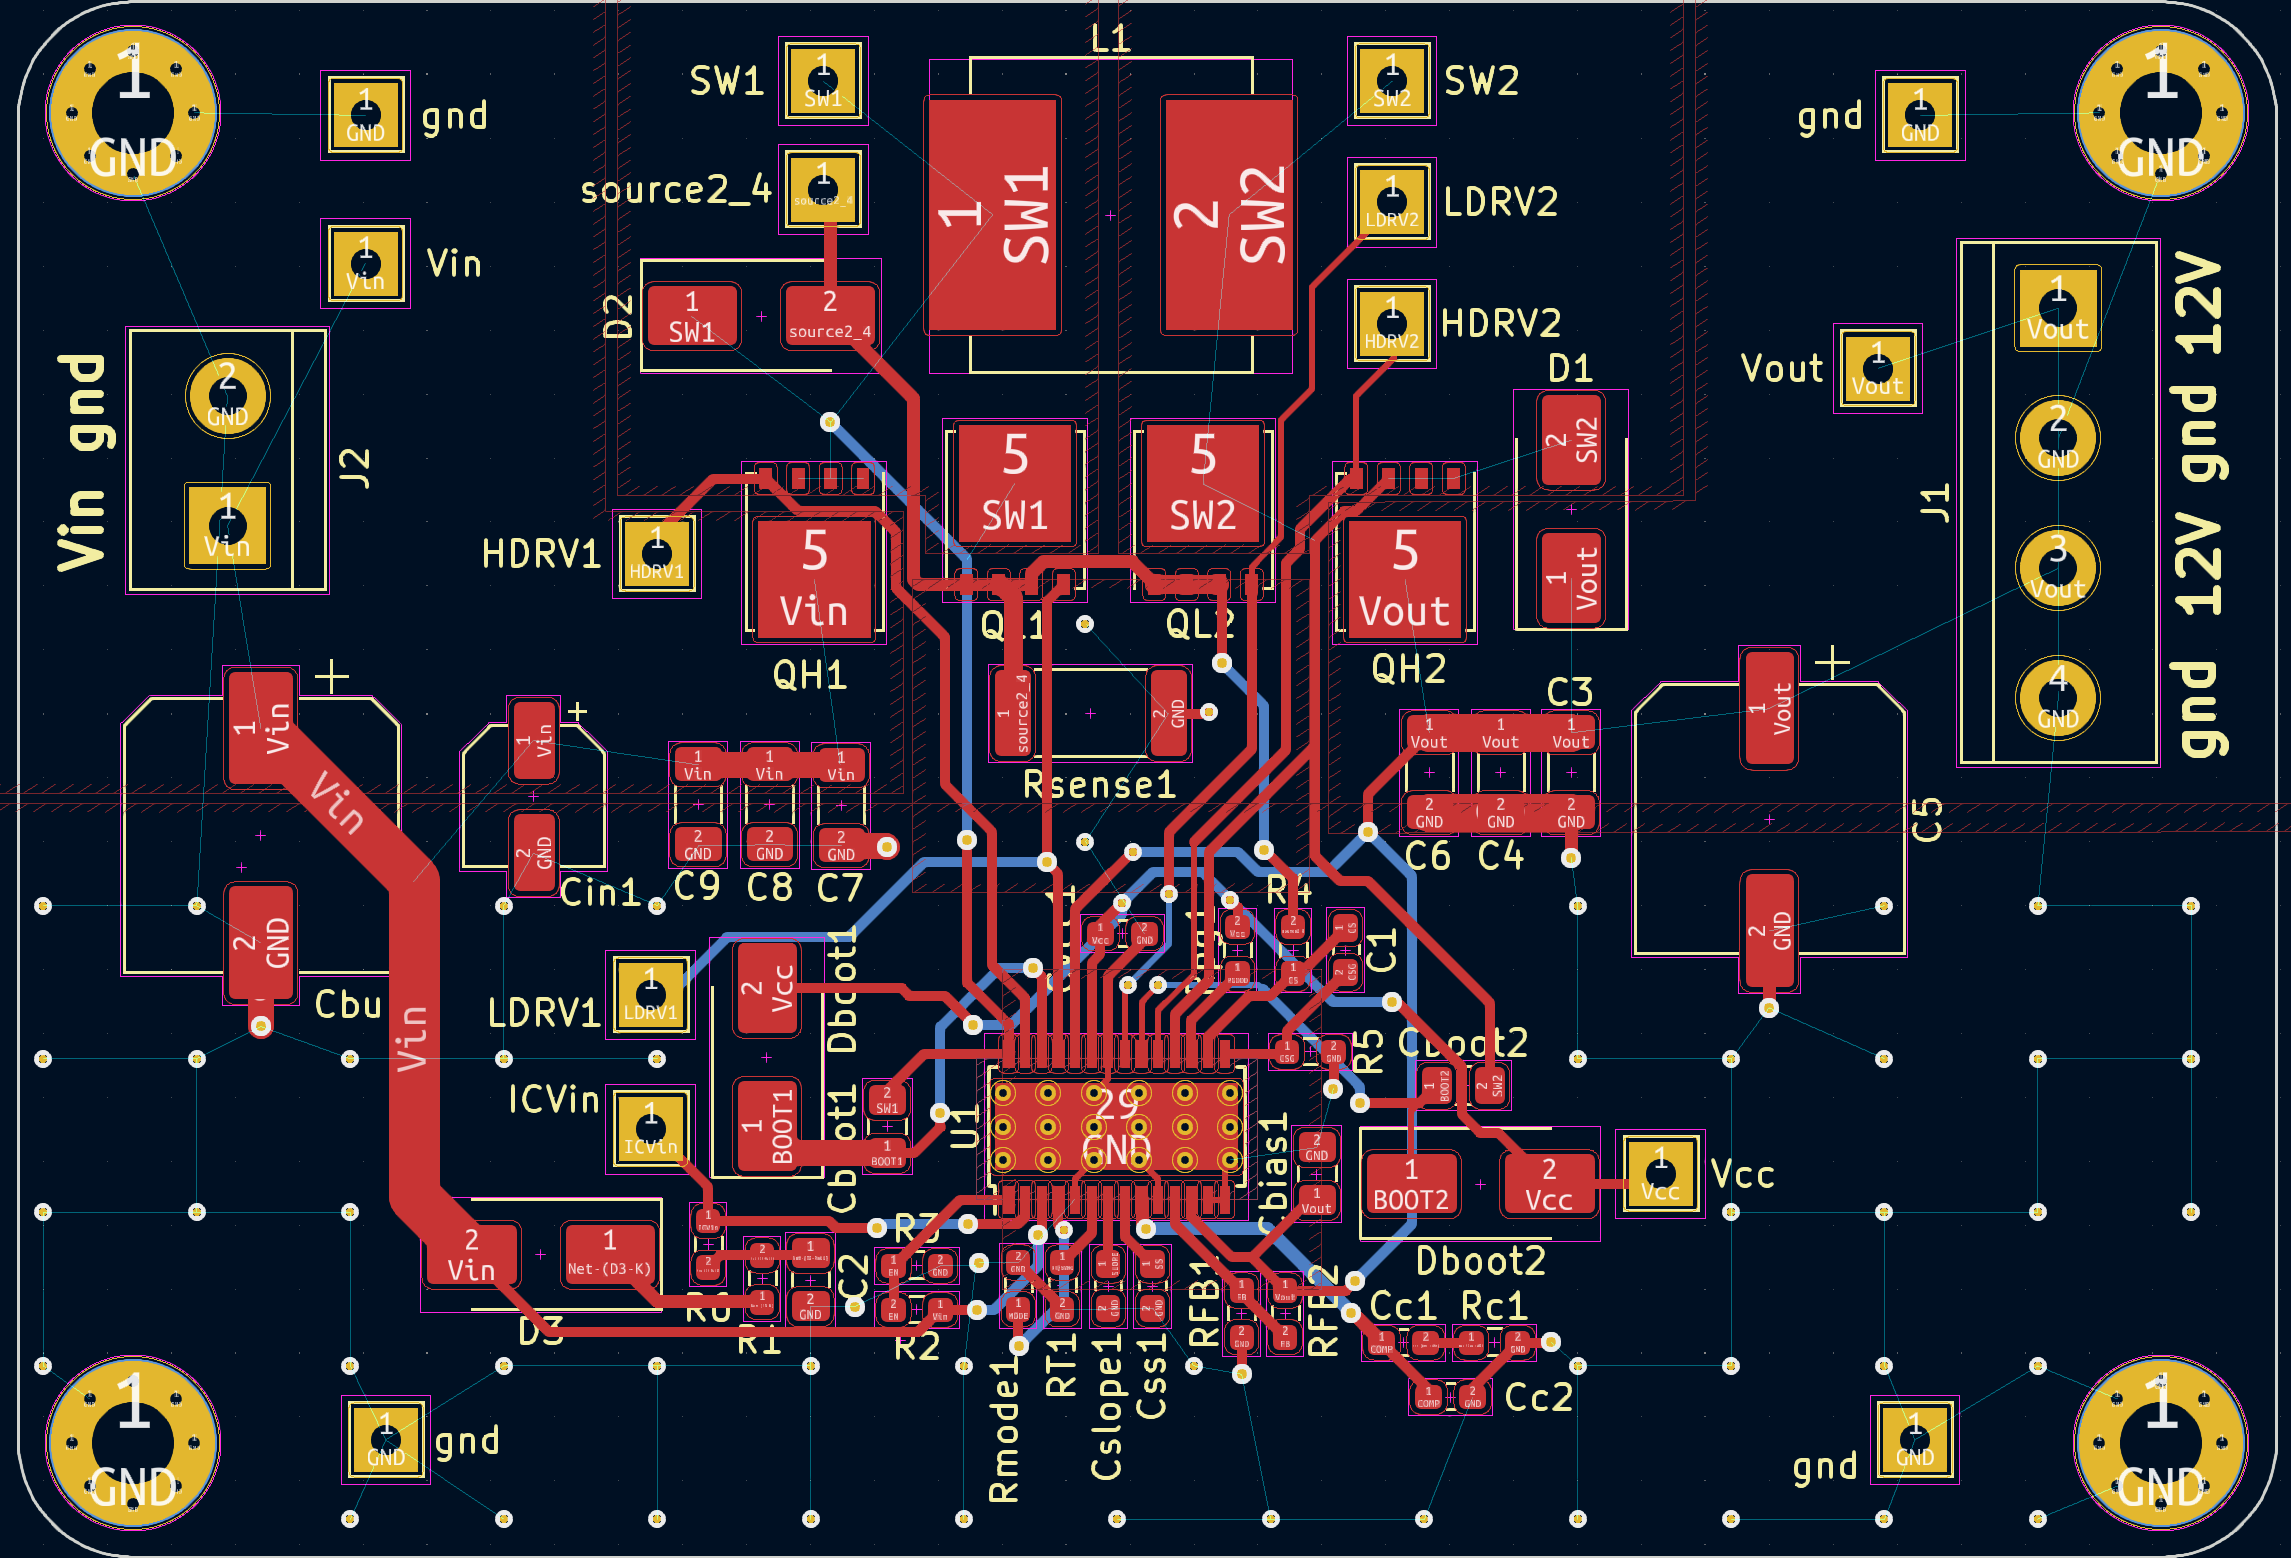
\includegraphics[width=\textwidth]{./figures/pcbLayers.png}
    \caption{PCB routing}
    \label{fig:pcbrouting}
\end{figure}

\newpage

In figures \ref{fig:pcbfront} and \ref{fig:pcbback}, 3D renders of the populated boards can be seen, while figure \ref{fig:assembledBoard} shows the final board fully assembled.

\begin{figure}[H]
    \centering
    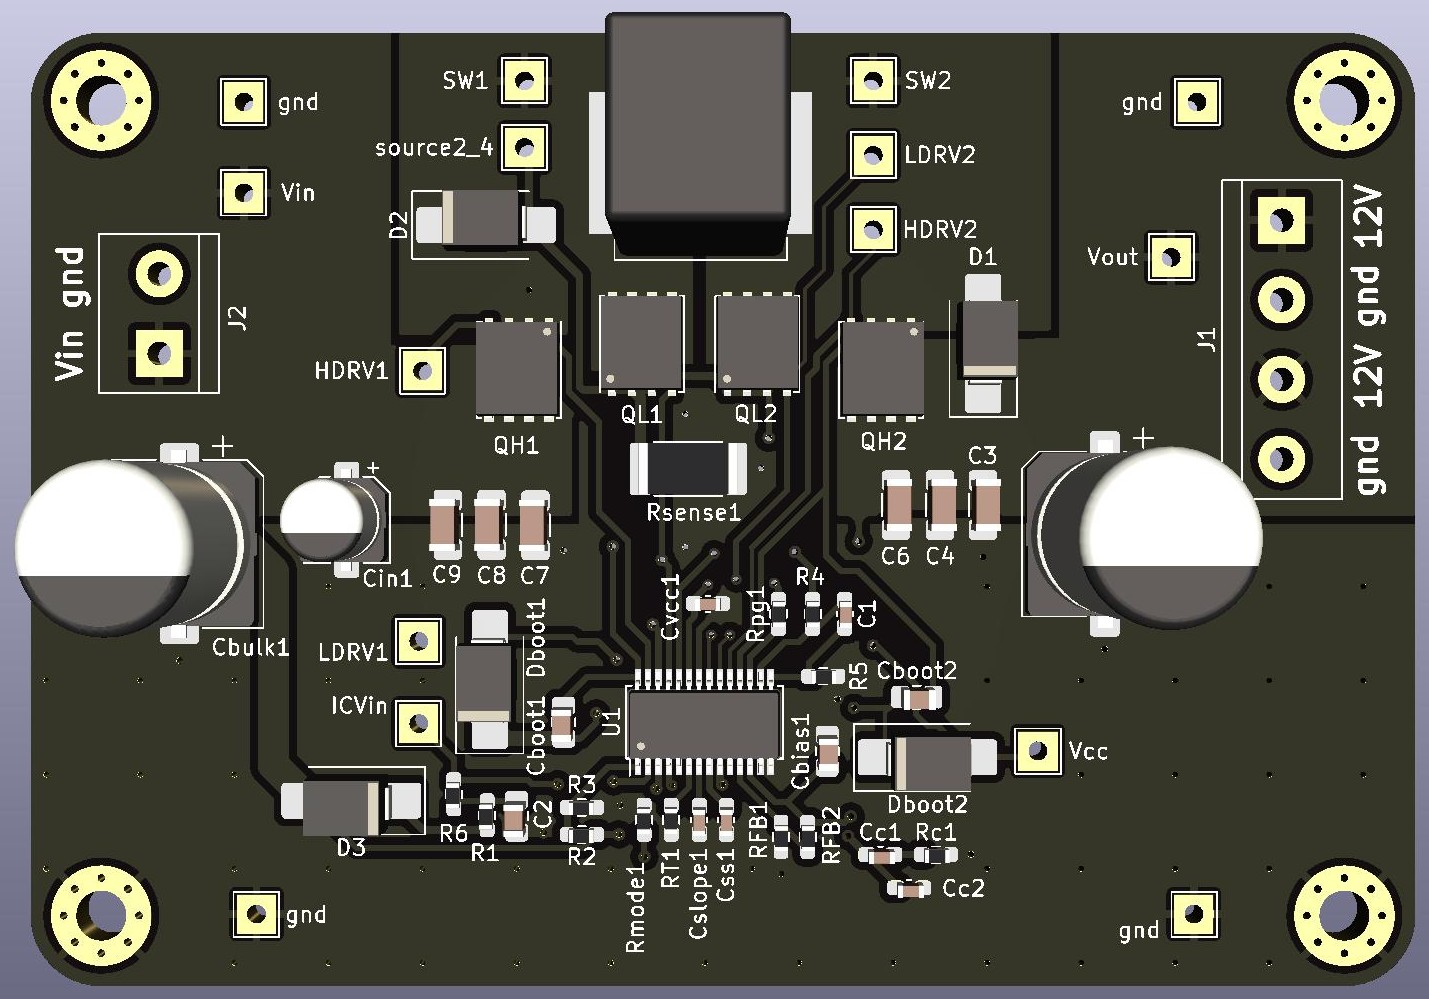
\includegraphics[width=0.9\textwidth]{./figures/pcbFront.jpg}
    \caption{Front of the PCB - 3D render}
    \label{fig:pcbfront}
\end{figure}

\begin{figure}[H]
    \centering
    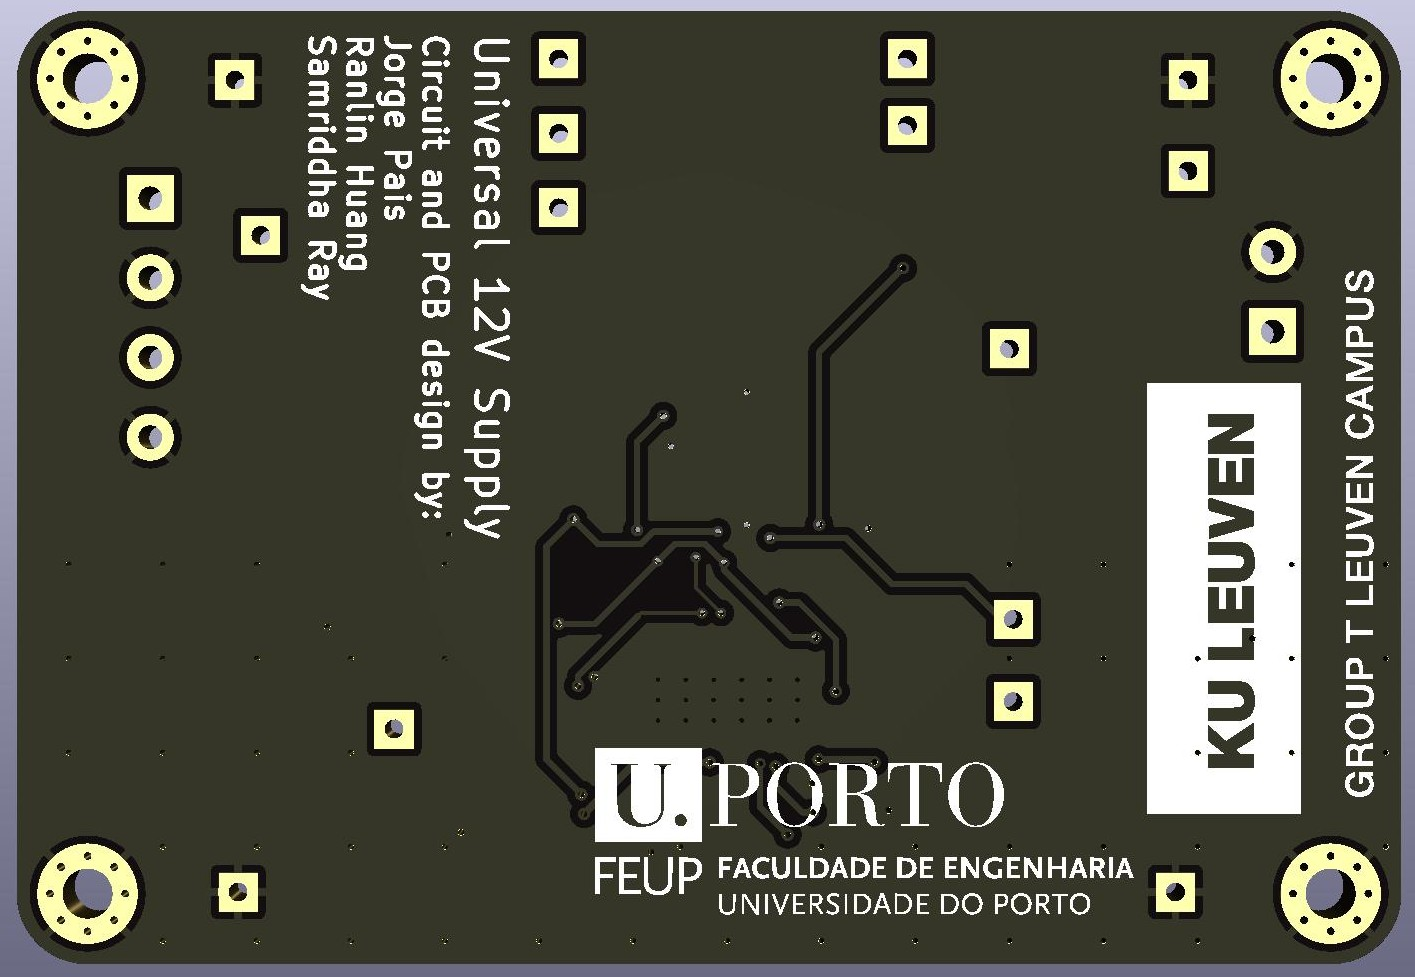
\includegraphics[width=0.9\textwidth]{./figures/pcbBack.jpg}
    \caption{Back of the PCB - 3D render}
    \label{fig:pcbback}
\end{figure}

Building the board was a matter of first laying solder paste across all SMD connections, carefully placing the components using tweezers and finally baking everything in the oven. The testpoints were then populated with small lugs which were hand soldered.

\begin{figure}[H]
    \centering
    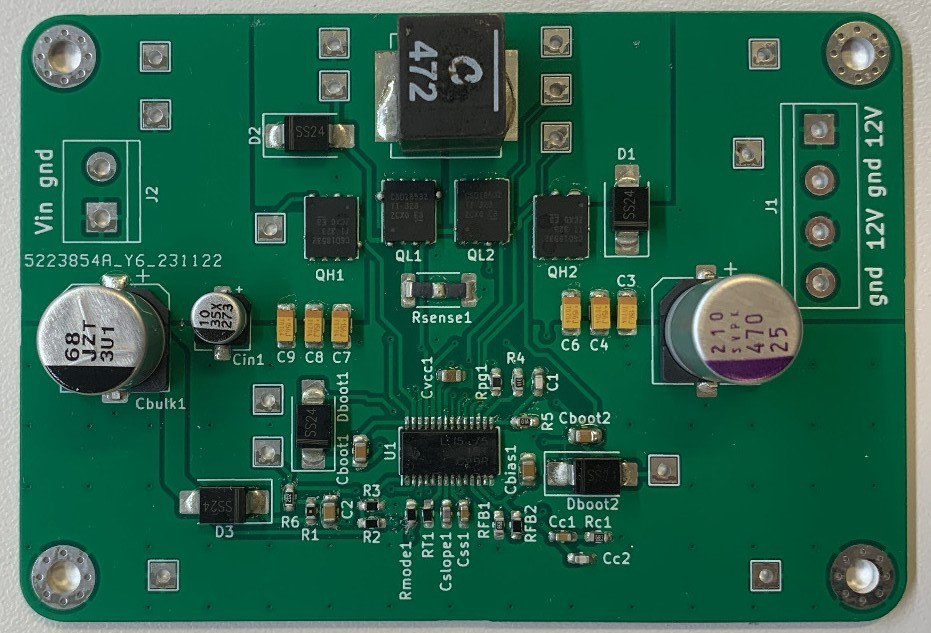
\includegraphics[width=\textwidth]{./figures/assembledBoard.jpg}
    \caption{Final assembled board}
    \label{fig:assembledBoard}
\end{figure}

\section{Measurements}

\vfill \pagebreak
\printbibliography

\vfill \pagebreak


\begin{appendices}
    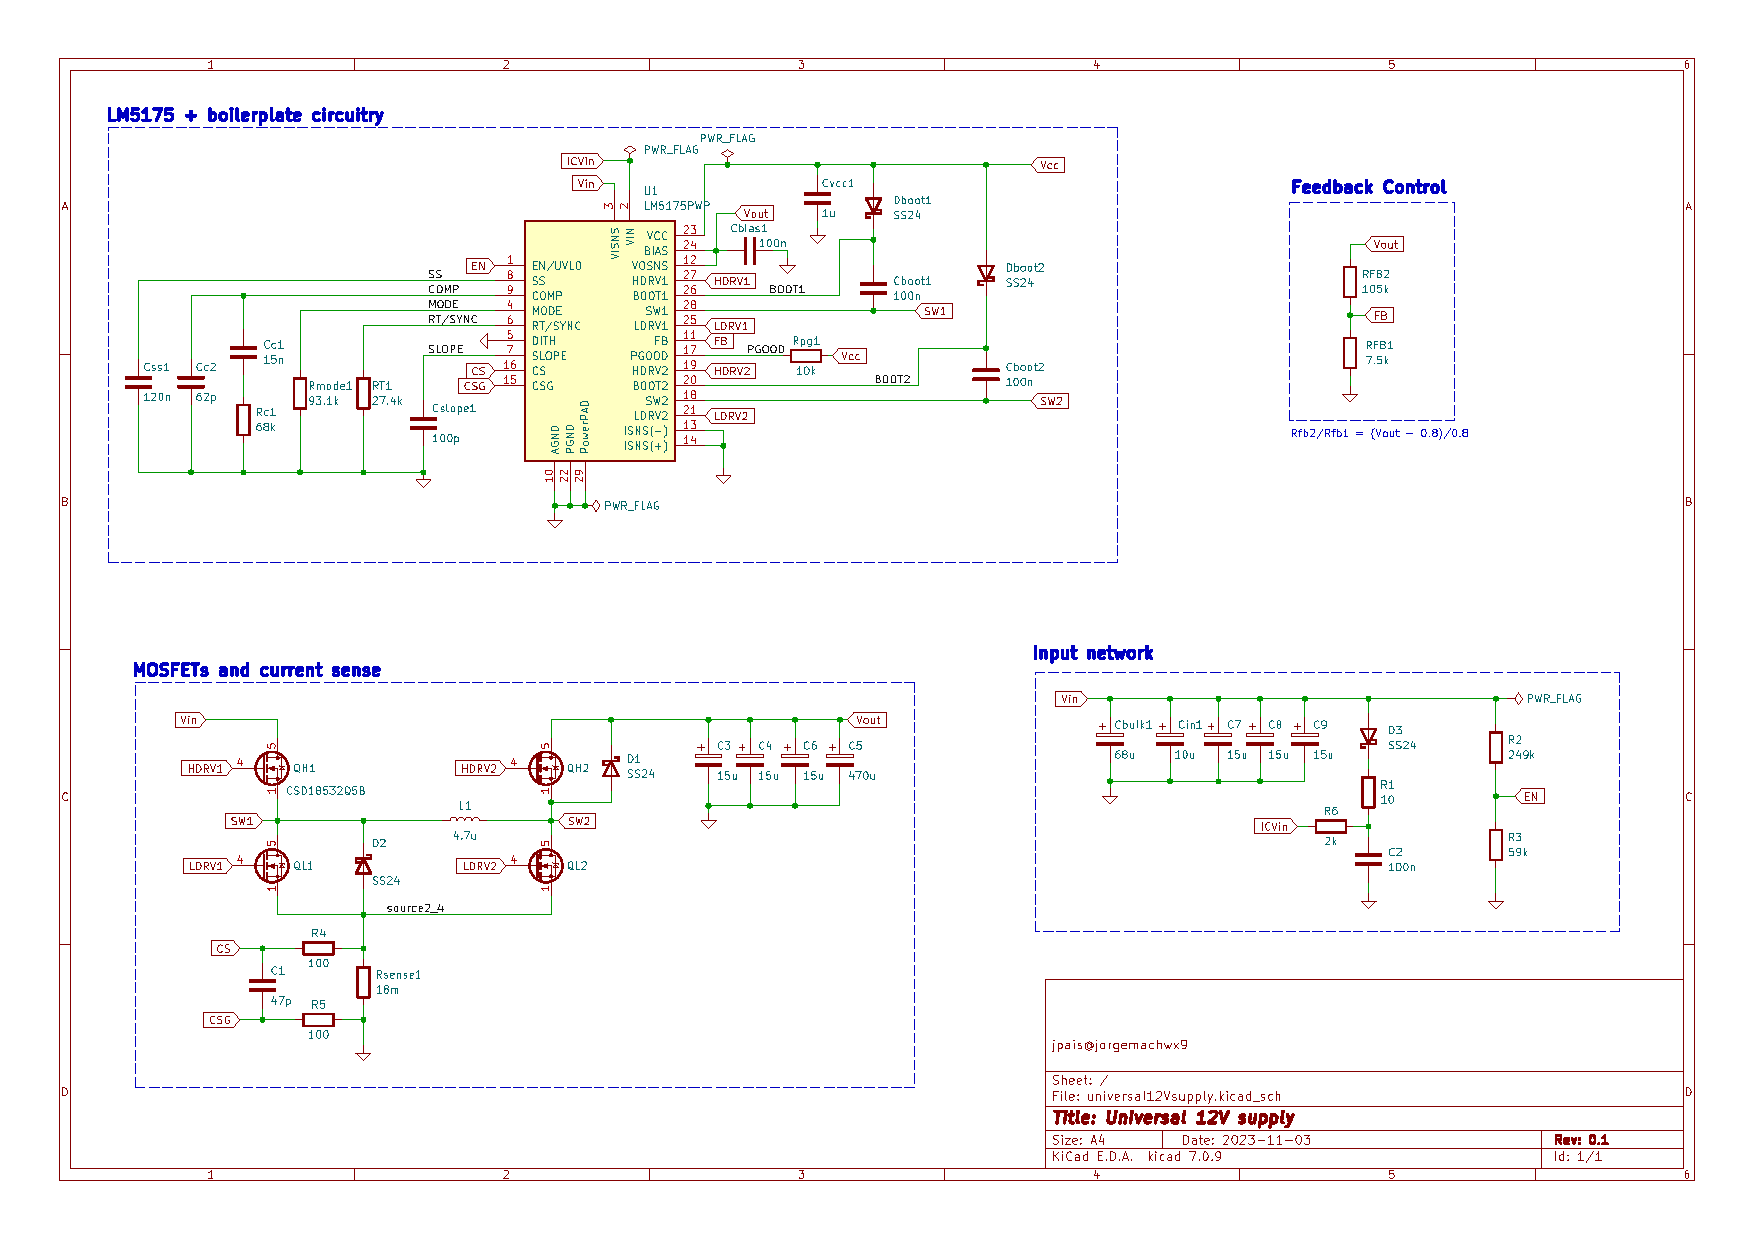
\includepdf[scale=1, fitpaper, angle=90]{./schematicSimple.pdf}
    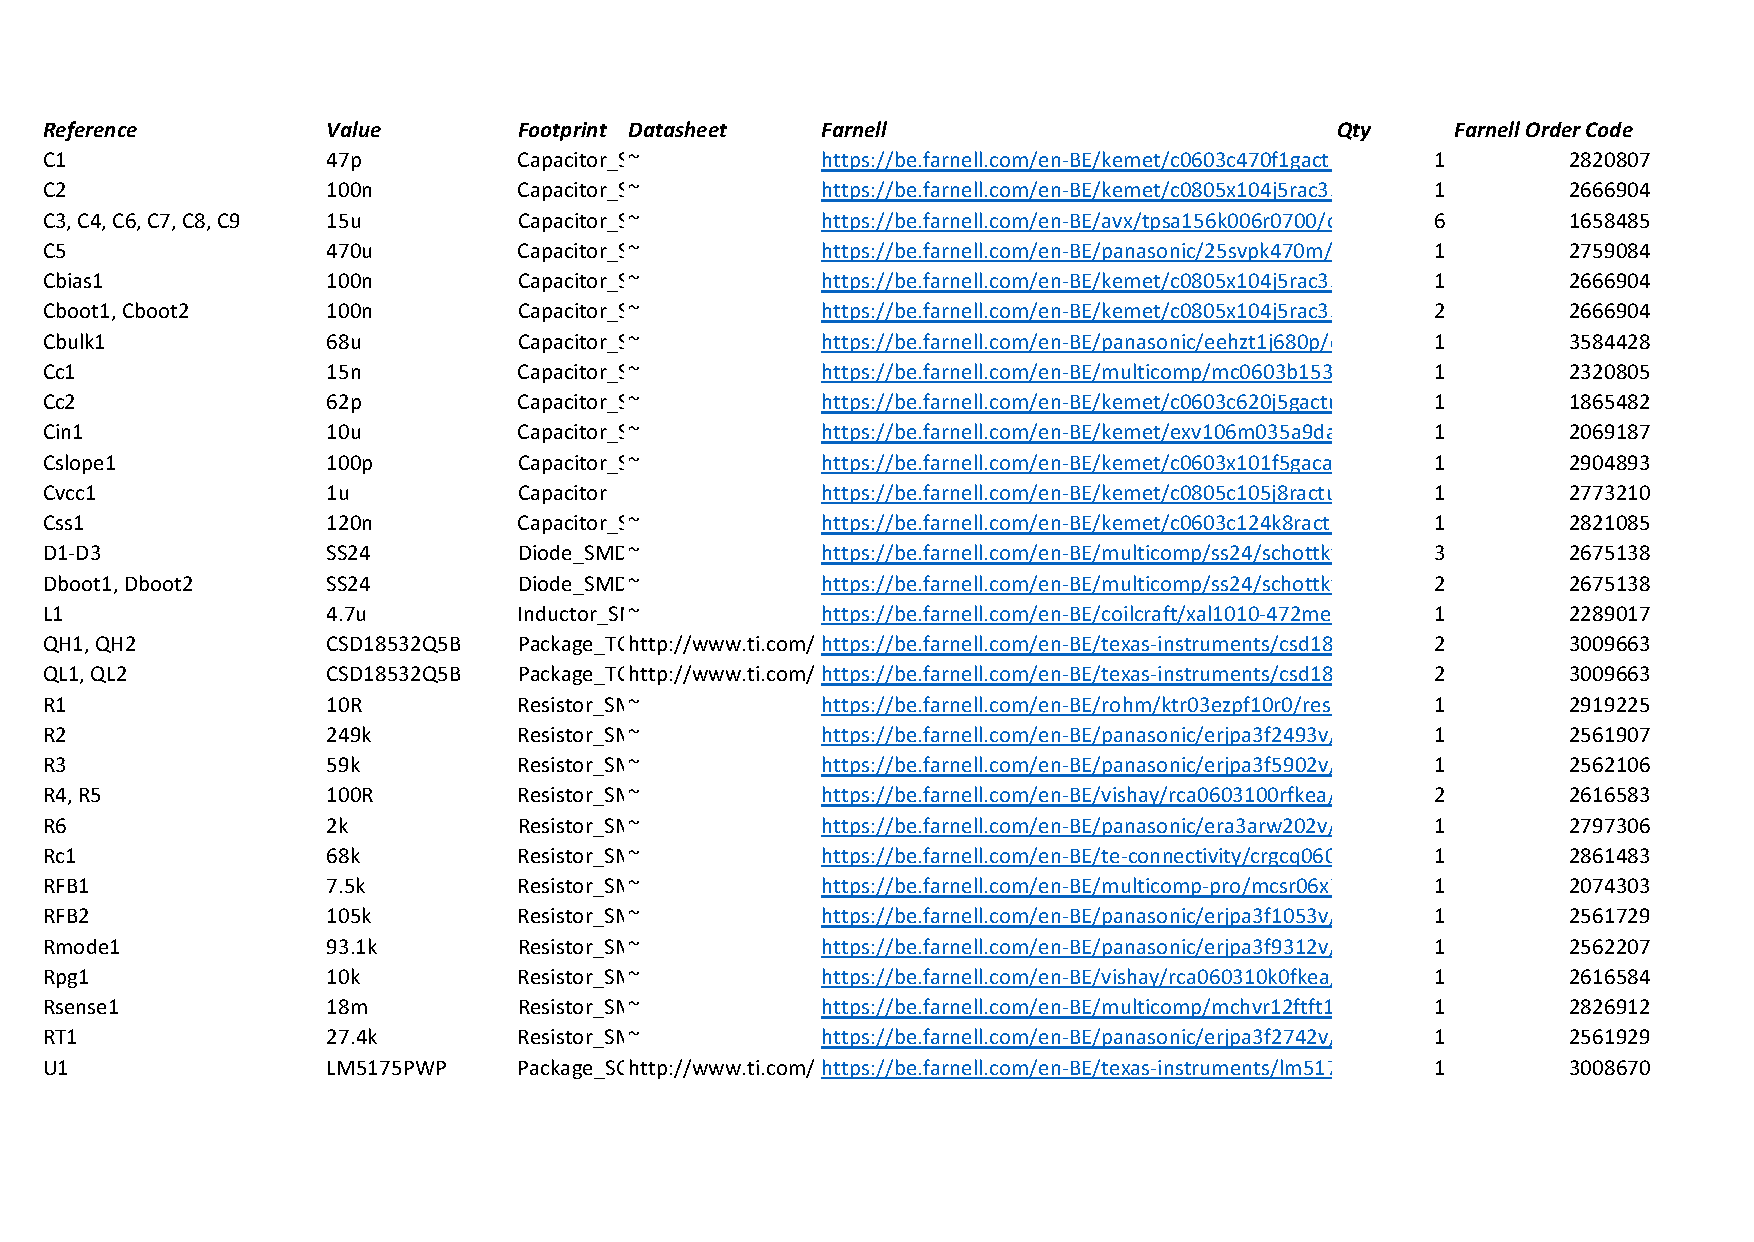
\includepdf[scale=1, fitpaper, angle=90]{./BOM.pdf}
\end{appendices}

\end{document}